\documentclass[1p]{elsarticle_modified}
%\bibliographystyle{elsarticle-num}

%\usepackage[colorlinks]{hyperref}
%\usepackage{abbrmath_seonhwa} %\Abb, \Ascr, \Acal ,\Abf, \Afrak
\usepackage{amsfonts}
\usepackage{amssymb}
\usepackage{amsmath}
\usepackage{amsthm}
\usepackage{scalefnt}
\usepackage{amsbsy}
\usepackage{kotex}
\usepackage{caption}
\usepackage{subfig}
\usepackage{color}
\usepackage{graphicx}
\usepackage{xcolor} %% white, black, red, green, blue, cyan, magenta, yellow
\usepackage{float}
\usepackage{setspace}
\usepackage{hyperref}

\usepackage{tikz}
\usetikzlibrary{arrows}

\usepackage{multirow}
\usepackage{array} % fixed length table
\usepackage{hhline}

%%%%%%%%%%%%%%%%%%%%%
\makeatletter
\renewcommand*\env@matrix[1][\arraystretch]{%
	\edef\arraystretch{#1}%
	\hskip -\arraycolsep
	\let\@ifnextchar\new@ifnextchar
	\array{*\c@MaxMatrixCols c}}
\makeatother %https://tex.stackexchange.com/questions/14071/how-can-i-increase-the-line-spacing-in-a-matrix
%%%%%%%%%%%%%%%

\usepackage[normalem]{ulem}

\newcommand{\msout}[1]{\ifmmode\text{\sout{\ensuremath{#1}}}\else\sout{#1}\fi}
%SOURCE: \msout is \stkout macro in https://tex.stackexchange.com/questions/20609/strikeout-in-math-mode

\newcommand{\cancel}[1]{
	\ifmmode
	{\color{red}\msout{#1}}
	\else
	{\color{red}\sout{#1}}
	\fi
}

\newcommand{\add}[1]{
	{\color{blue}\uwave{#1}}
}

\newcommand{\replace}[2]{
	\ifmmode
	{\color{red}\msout{#1}}{\color{blue}\uwave{#2}}
	\else
	{\color{red}\sout{#1}}{\color{blue}\uwave{#2}}
	\fi
}

\newcommand{\Sol}{\mathcal{S}} %segment
\newcommand{\D}{D} %diagram
\newcommand{\A}{\mathcal{A}} %arc


%%%%%%%%%%%%%%%%%%%%%%%%%%%%%5 test

\def\sl{\operatorname{\textup{SL}}(2,\Cbb)}
\def\psl{\operatorname{\textup{PSL}}(2,\Cbb)}
\def\quan{\mkern 1mu \triangleright \mkern 1mu}

\theoremstyle{definition}
\newtheorem{thm}{Theorem}[section]
\newtheorem{prop}[thm]{Proposition}
\newtheorem{lem}[thm]{Lemma}
\newtheorem{ques}[thm]{Question}
\newtheorem{cor}[thm]{Corollary}
\newtheorem{defn}[thm]{Definition}
\newtheorem{exam}[thm]{Example}
\newtheorem{rmk}[thm]{Remark}
\newtheorem{alg}[thm]{Algorithm}

\newcommand{\I}{\sqrt{-1}}
\begin{document}

%\begin{frontmatter}
%
%\title{Boundary parabolic representations of knots up to 8 crossings}
%
%%% Group authors per affiliation:
%\author{Yunhi Cho} 
%\address{Department of Mathematics, University of Seoul, Seoul, Korea}
%\ead{yhcho@uos.ac.kr}
%
%
%\author{Seonhwa Kim} %\fnref{s_kim}}
%\address{Center for Geometry and Physics, Institute for Basic Science, Pohang, 37673, Korea}
%\ead{ryeona17@ibs.re.kr}
%
%\author{Hyuk Kim}
%\address{Department of Mathematical Sciences, Seoul National University, Seoul 08826, Korea}
%\ead{hyukkim@snu.ac.kr}
%
%\author{Seokbeom Yoon}
%\address{Department of Mathematical Sciences, Seoul National University, Seoul, 08826,  Korea}
%\ead{sbyoon15@snu.ac.kr}
%
%\begin{abstract}
%We find all boundary parabolic representation of knots up to 8 crossings.
%
%\end{abstract}
%\begin{keyword}
%    \MSC[2010] 57M25 
%\end{keyword}
%
%\end{frontmatter}

%\linenumbers
%\tableofcontents
%
\newcommand\colored[1]{\textcolor{white}{\rule[-0.35ex]{0.8em}{1.4ex}}\kern-0.8em\color{red} #1}%
%\newcommand\colored[1]{\textcolor{white}{ #1}\kern-2.17ex	\textcolor{white}{ #1}\kern-1.81ex	\textcolor{white}{ #1}\kern-2.15ex\color{red}#1	}

{\Large $\underline{12a_{0069}~(K12a_{0069})}$}

\setlength{\tabcolsep}{10pt}
\renewcommand{\arraystretch}{1.6}
\vspace{1cm}\begin{tabular}{m{100pt}>{\centering\arraybackslash}m{274pt}}
\multirow{5}{120pt}{
	\centering
	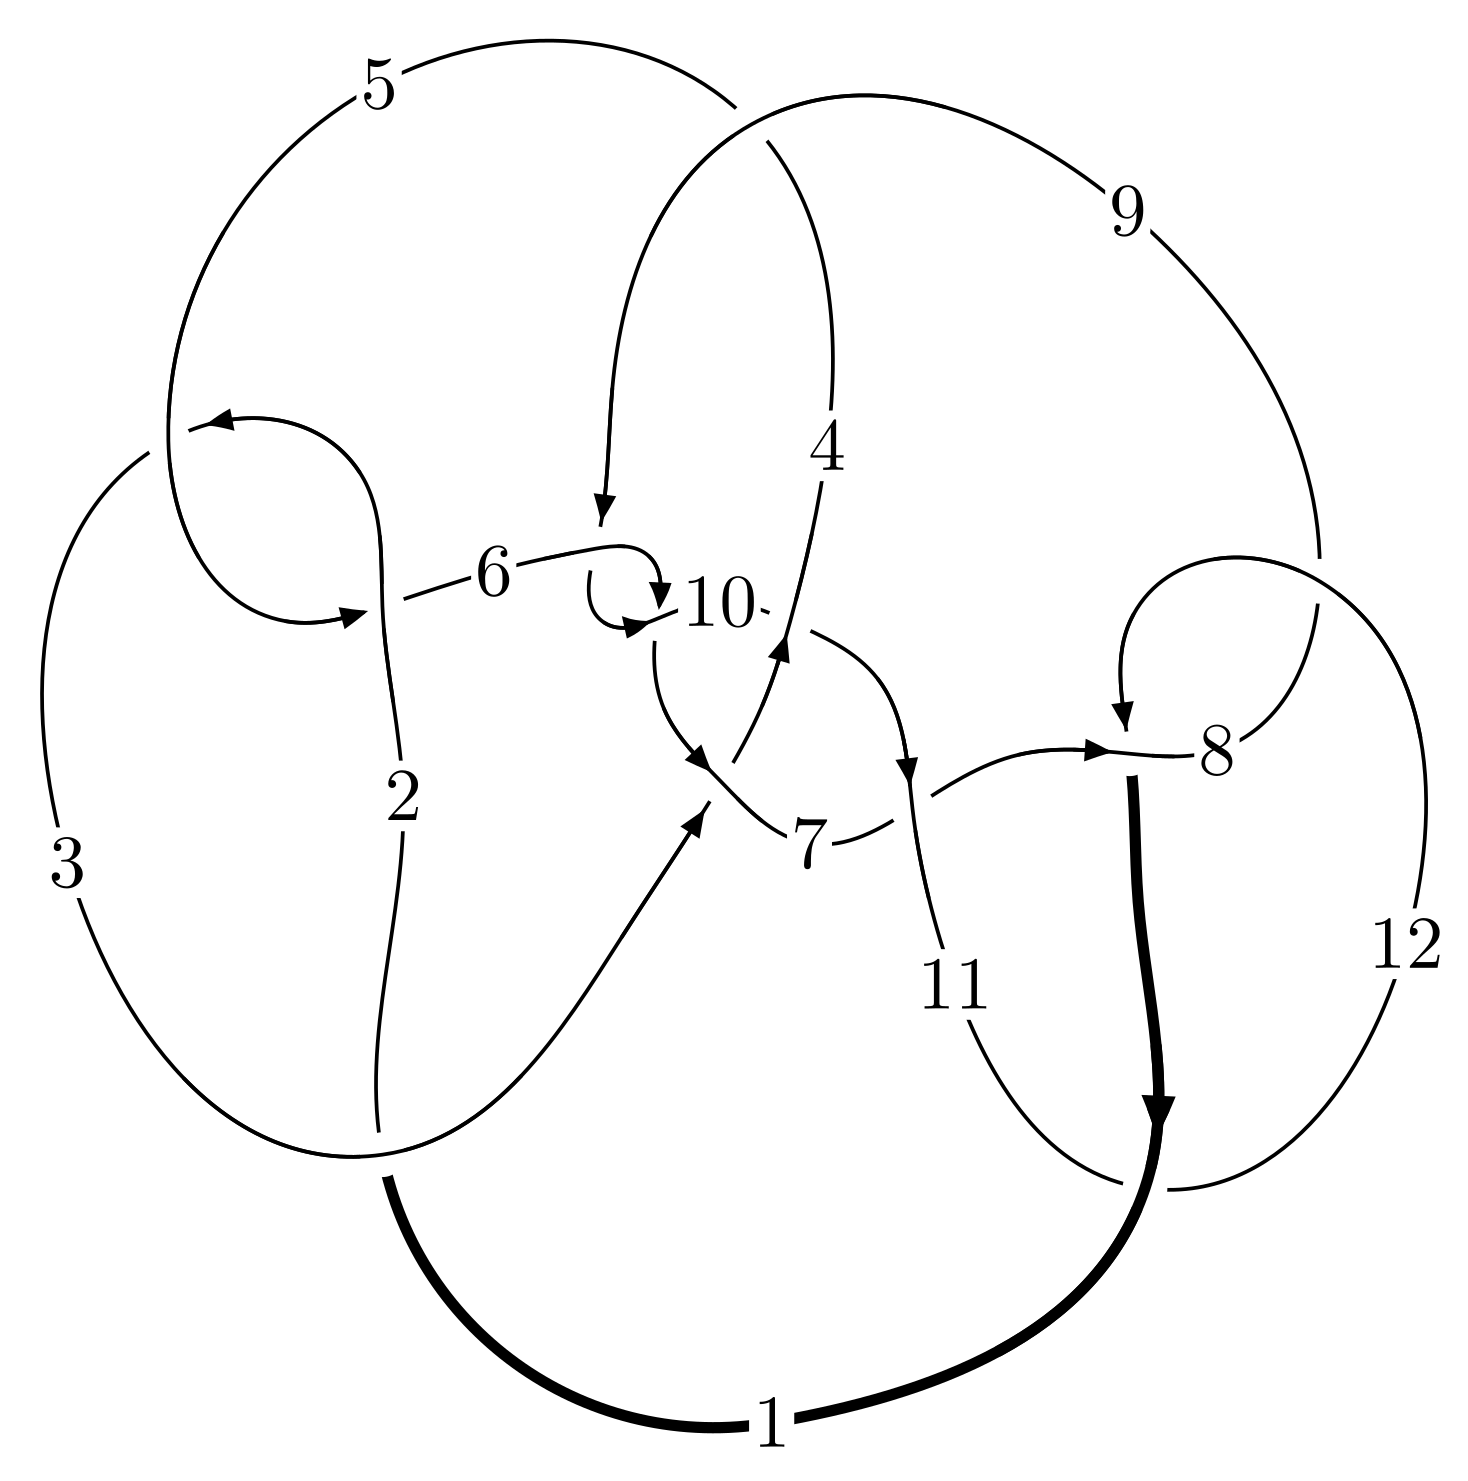
\includegraphics[width=112pt]{../../../GIT/diagram.site/Diagrams/png/870_12a_0069.png}\\
\ \ \ A knot diagram\footnotemark}&
\allowdisplaybreaks
\textbf{Linearized knot diagam} \\
\cline{2-2}
 &
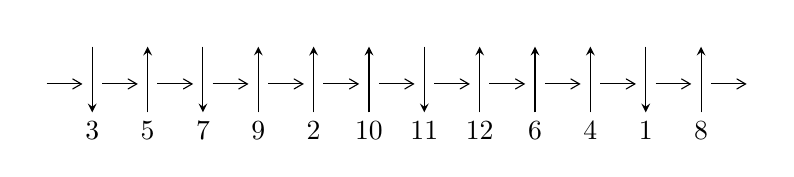
\begin{tikzpicture}[x=20pt, y=17pt]
	% nodes
	\node (C0) at (0, 0) {};
	\node (C1) at (1, 0) {};
	\node (C1U) at (1, +1) {};
	\node (C1D) at (1, -1) {3};

	\node (C2) at (2, 0) {};
	\node (C2U) at (2, +1) {};
	\node (C2D) at (2, -1) {5};

	\node (C3) at (3, 0) {};
	\node (C3U) at (3, +1) {};
	\node (C3D) at (3, -1) {7};

	\node (C4) at (4, 0) {};
	\node (C4U) at (4, +1) {};
	\node (C4D) at (4, -1) {9};

	\node (C5) at (5, 0) {};
	\node (C5U) at (5, +1) {};
	\node (C5D) at (5, -1) {2};

	\node (C6) at (6, 0) {};
	\node (C6U) at (6, +1) {};
	\node (C6D) at (6, -1) {10};

	\node (C7) at (7, 0) {};
	\node (C7U) at (7, +1) {};
	\node (C7D) at (7, -1) {11};

	\node (C8) at (8, 0) {};
	\node (C8U) at (8, +1) {};
	\node (C8D) at (8, -1) {12};

	\node (C9) at (9, 0) {};
	\node (C9U) at (9, +1) {};
	\node (C9D) at (9, -1) {6};

	\node (C10) at (10, 0) {};
	\node (C10U) at (10, +1) {};
	\node (C10D) at (10, -1) {4};

	\node (C11) at (11, 0) {};
	\node (C11U) at (11, +1) {};
	\node (C11D) at (11, -1) {1};

	\node (C12) at (12, 0) {};
	\node (C12U) at (12, +1) {};
	\node (C12D) at (12, -1) {8};
	\node (C13) at (13, 0) {};

	% arrows
	\draw[->,>={angle 60}]
	(C0) edge (C1) (C1) edge (C2) (C2) edge (C3) (C3) edge (C4) (C4) edge (C5) (C5) edge (C6) (C6) edge (C7) (C7) edge (C8) (C8) edge (C9) (C9) edge (C10) (C10) edge (C11) (C11) edge (C12) (C12) edge (C13) ;	\draw[->,>=stealth]
	(C1U) edge (C1D) (C2D) edge (C2U) (C3U) edge (C3D) (C4D) edge (C4U) (C5D) edge (C5U) (C6D) edge (C6U) (C7U) edge (C7D) (C8D) edge (C8U) (C9D) edge (C9U) (C10D) edge (C10U) (C11U) edge (C11D) (C12D) edge (C12U) ;
	\end{tikzpicture} \\
\hhline{~~} \\& 
\textbf{Solving Sequence} \\ \cline{2-2} 
 &
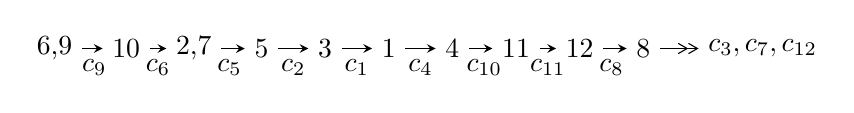
\begin{tikzpicture}[x=23pt, y=7pt]
	% node
	\node (A0) at (-1/8, 0) {6,9};
	\node (A1) at (1, 0) {10};
	\node (A2) at (33/16, 0) {2,7};
	\node (A3) at (25/8, 0) {5};
	\node (A4) at (33/8, 0) {3};
	\node (A5) at (41/8, 0) {1};
	\node (A6) at (49/8, 0) {4};
	\node (A7) at (57/8, 0) {11};
	\node (A8) at (65/8, 0) {12};
	\node (A9) at (73/8, 0) {8};
	\node (C1) at (1/2, -1) {$c_{9}$};
	\node (C2) at (3/2, -1) {$c_{6}$};
	\node (C3) at (21/8, -1) {$c_{5}$};
	\node (C4) at (29/8, -1) {$c_{2}$};
	\node (C5) at (37/8, -1) {$c_{1}$};
	\node (C6) at (45/8, -1) {$c_{4}$};
	\node (C7) at (53/8, -1) {$c_{10}$};
	\node (C8) at (61/8, -1) {$c_{11}$};
	\node (C9) at (69/8, -1) {$c_{8}$};
	\node (A10) at (11, 0) {$c_{3},c_{7},c_{12}$};

	% edge
	\draw[->,>=stealth]	
	(A0) edge (A1) (A1) edge (A2) (A2) edge (A3) (A3) edge (A4) (A4) edge (A5) (A5) edge (A6) (A6) edge (A7) (A7) edge (A8) (A8) edge (A9) ;
	\draw[->>,>={angle 60}]	
	(A9) edge (A10);
\end{tikzpicture} \\ 

\end{tabular} \\

\footnotetext{
The image of knot diagram is generated by the software ``\textbf{Draw programme}" developed by Andrew Bartholomew(\url{http://www.layer8.co.uk/maths/draw/index.htm\#Running-draw}), where we modified some parts for our purpose(\url{https://github.com/CATsTAILs/LinksPainter}).
}\phantom \\ \newline 
\centering \textbf{Ideals for irreducible components\footnotemark of $X_{\text{par}}$} 
 
\begin{align*}
I^u_{1}&=\langle 
7.65770\times10^{416} u^{118}-1.62086\times10^{417} u^{117}+\cdots+7.02397\times10^{415} b-9.50919\times10^{416},\\
\phantom{I^u_{1}}&\phantom{= \langle  }-7.94572\times10^{415} u^{118}+1.92807\times10^{416} u^{117}+\cdots+7.02397\times10^{415} a+1.46155\times10^{416},\\
\phantom{I^u_{1}}&\phantom{= \langle  }u^{119}- u^{118}+\cdots-10 u^3-1\rangle \\
\\
\end{align*}
\raggedright * 1 irreducible components of $\dim_{\mathbb{C}}=0$, with total 119 representations.\\
\footnotetext{All coefficients of polynomials are rational numbers. But the coefficients are sometimes approximated in decimal forms when there is not enough margin.}
\newpage
\renewcommand{\arraystretch}{1}
\centering \section*{I. $I^u_{1}= \langle 7.66\times10^{416} u^{118}-1.62\times10^{417} u^{117}+\cdots+7.02\times10^{415} b-9.51\times10^{416},\;-7.95\times10^{415} u^{118}+1.93\times10^{416} u^{117}+\cdots+7.02\times10^{415} a+1.46\times10^{416},\;u^{119}- u^{118}+\cdots-10 u^3-1 \rangle$}
\flushleft \textbf{(i) Arc colorings}\\
\begin{tabular}{m{7pt} m{180pt} m{7pt} m{180pt} }
\flushright $a_{6}=$&$\begin{pmatrix}0\\u\end{pmatrix}$ \\
\flushright $a_{9}=$&$\begin{pmatrix}1\\0\end{pmatrix}$ \\
\flushright $a_{10}=$&$\begin{pmatrix}1\\- u^2\end{pmatrix}$ \\
\flushright $a_{2}=$&$\begin{pmatrix}1.13123 u^{118}-2.74499 u^{117}+\cdots-0.679206 u-2.08080\\-10.9022 u^{118}+23.0761 u^{117}+\cdots-11.1828 u+13.5382\end{pmatrix}$ \\
\flushright $a_{7}=$&$\begin{pmatrix}u\\- u^3+u\end{pmatrix}$ \\
\flushright $a_{5}=$&$\begin{pmatrix}0.947849 u^{118}-3.85311 u^{117}+\cdots-3.86697 u-3.09518\\-14.8208 u^{118}+24.3819 u^{117}+\cdots-16.3486 u+11.6263\end{pmatrix}$ \\
\flushright $a_{3}=$&$\begin{pmatrix}0.869184 u^{118}-4.24063 u^{117}+\cdots-4.92860 u-3.11758\\-15.6125 u^{118}+27.9535 u^{117}+\cdots-18.8594 u+14.1353\end{pmatrix}$ \\
\flushright $a_{1}=$&$\begin{pmatrix}-0.700733 u^{118}-0.837427 u^{117}+\cdots+2.27817 u-0.562810\\0.130477 u^{118}+1.80102 u^{117}+\cdots-2.77571 u+1.78291\end{pmatrix}$ \\
\flushright $a_{4}=$&$\begin{pmatrix}15.7687 u^{118}-28.2350 u^{117}+\cdots+12.4817 u-14.7215\\-14.8208 u^{118}+24.3819 u^{117}+\cdots-16.3486 u+11.6263\end{pmatrix}$ \\
\flushright $a_{11}=$&$\begin{pmatrix}0.244750 u^{118}-1.71369 u^{117}+\cdots-1.10194 u-3.47644\\-1.42573 u^{118}+1.50735 u^{117}+\cdots-0.807561 u+0.768205\end{pmatrix}$ \\
\flushright $a_{12}=$&$\begin{pmatrix}0.683348 u^{118}-1.40205 u^{117}+\cdots-0.666971 u-2.50037\\2.26430 u^{118}-3.52278 u^{117}+\cdots+2.98299 u-1.11611\end{pmatrix}$ \\
\flushright $a_{8}=$&$\begin{pmatrix}-3.44836 u^{118}+3.50134 u^{117}+\cdots-5.29495 u+0.898973\\3.52208 u^{118}-3.23364 u^{117}+\cdots+4.70691 u-0.312411\end{pmatrix}$\\&\end{tabular}
\flushleft \textbf{(ii) Obstruction class $= -1$}\\~\\
\flushleft \textbf{(iii) Cusp Shapes $= -91.5861 u^{118}+200.489 u^{117}+\cdots-97.6537 u+125.725$}\\~\\
\newpage\renewcommand{\arraystretch}{1}
\flushleft \textbf{(iv) u-Polynomials at the component}\newline \\
\begin{tabular}{m{50pt}|m{274pt}}
Crossings & \hspace{64pt}u-Polynomials at each crossing \\
\hline $$\begin{aligned}c_{1}\end{aligned}$$&$\begin{aligned}
&u^{119}+47 u^{118}+\cdots+76 u-1
\end{aligned}$\\
\hline $$\begin{aligned}c_{2},c_{5}\end{aligned}$$&$\begin{aligned}
&u^{119}+u^{118}+\cdots+4 u-1
\end{aligned}$\\
\hline $$\begin{aligned}c_{3}\end{aligned}$$&$\begin{aligned}
&u^{119}-11 u^{118}+\cdots-44 u-41
\end{aligned}$\\
\hline $$\begin{aligned}c_{4}\end{aligned}$$&$\begin{aligned}
&u^{119}+17 u^{118}+\cdots-9590288 u-2011573
\end{aligned}$\\
\hline $$\begin{aligned}c_{6},c_{9}\end{aligned}$$&$\begin{aligned}
&u^{119}- u^{118}+\cdots-10 u^3-1
\end{aligned}$\\
\hline $$\begin{aligned}c_{7}\end{aligned}$$&$\begin{aligned}
&u^{119}+5 u^{118}+\cdots-2541506 u-300233
\end{aligned}$\\
\hline $$\begin{aligned}c_{8},c_{12}\end{aligned}$$&$\begin{aligned}
&u^{119}-5 u^{118}+\cdots+2 u-1
\end{aligned}$\\
\hline $$\begin{aligned}c_{10}\end{aligned}$$&$\begin{aligned}
&u^{119}-3 u^{118}+\cdots-4 u+1
\end{aligned}$\\
\hline $$\begin{aligned}c_{11}\end{aligned}$$&$\begin{aligned}
&u^{119}+59 u^{118}+\cdots-10 u^2-1
\end{aligned}$\\
\hline
\end{tabular}\\~\\
\newpage\renewcommand{\arraystretch}{1}
\flushleft \textbf{(v) Riley Polynomials at the component}\newline \\
\begin{tabular}{m{50pt}|m{274pt}}
Crossings & \hspace{64pt}Riley Polynomials at each crossing \\
\hline $$\begin{aligned}c_{1}\end{aligned}$$&$\begin{aligned}
&y^{119}+51 y^{118}+\cdots+3612 y-1
\end{aligned}$\\
\hline $$\begin{aligned}c_{2},c_{5}\end{aligned}$$&$\begin{aligned}
&y^{119}+47 y^{118}+\cdots+76 y-1
\end{aligned}$\\
\hline $$\begin{aligned}c_{3}\end{aligned}$$&$\begin{aligned}
&y^{119}-29 y^{118}+\cdots-1094568 y-1681
\end{aligned}$\\
\hline $$\begin{aligned}c_{4}\end{aligned}$$&$\begin{aligned}
&y^{119}-97 y^{118}+\cdots+36045891989112 y-4046425934329
\end{aligned}$\\
\hline $$\begin{aligned}c_{6},c_{9}\end{aligned}$$&$\begin{aligned}
&y^{119}-85 y^{118}+\cdots+10 y^2-1
\end{aligned}$\\
\hline $$\begin{aligned}c_{7}\end{aligned}$$&$\begin{aligned}
&y^{119}-53 y^{118}+\cdots-333755460568 y-90139854289
\end{aligned}$\\
\hline $$\begin{aligned}c_{8},c_{12}\end{aligned}$$&$\begin{aligned}
&y^{119}+59 y^{118}+\cdots-10 y^2-1
\end{aligned}$\\
\hline $$\begin{aligned}c_{10}\end{aligned}$$&$\begin{aligned}
&y^{119}-5 y^{118}+\cdots+36 y-1
\end{aligned}$\\
\hline $$\begin{aligned}c_{11}\end{aligned}$$&$\begin{aligned}
&y^{119}+3 y^{118}+\cdots-20 y-1
\end{aligned}$\\
\hline
\end{tabular}\\~\\
\newpage\flushleft \textbf{(vi) Complex Volumes and Cusp Shapes}
$$\begin{array}{c|c|c}  
\text{Solutions to }I^u_{1}& \I (\text{vol} + \sqrt{-1}CS) & \text{Cusp shape}\\
 \hline 
\begin{aligned}
u &= -1.035610 + 0.034259 I \\
a &= \phantom{-}0.442668 + 0.851761 I \\
b &= -3.97968 + 9.10996 I\end{aligned}
 & -0.86467 - 1.64898 I & \phantom{-0.000000 } 0 \\ \hline\begin{aligned}
u &= -1.035610 - 0.034259 I \\
a &= \phantom{-}0.442668 - 0.851761 I \\
b &= -3.97968 - 9.10996 I\end{aligned}
 & -0.86467 + 1.64898 I & \phantom{-0.000000 } 0 \\ \hline\begin{aligned}
u &= -0.153531 + 0.943119 I \\
a &= \phantom{-}0.329336 - 0.874707 I \\
b &= \phantom{-}0.612984 - 0.109115 I\end{aligned}
 & -2.01394 - 8.29603 I & \phantom{-0.000000 } 0 \\ \hline\begin{aligned}
u &= -0.153531 - 0.943119 I \\
a &= \phantom{-}0.329336 + 0.874707 I \\
b &= \phantom{-}0.612984 + 0.109115 I\end{aligned}
 & -2.01394 + 8.29603 I & \phantom{-0.000000 } 0 \\ \hline\begin{aligned}
u &= \phantom{-}0.195630 + 0.932978 I \\
a &= -0.333343 - 0.813020 I \\
b &= -0.621938 + 0.026733 I\end{aligned}
 & \phantom{-}0.44663 + 3.21872 I & \phantom{-0.000000 } 0 \\ \hline\begin{aligned}
u &= \phantom{-}0.195630 - 0.932978 I \\
a &= -0.333343 + 0.813020 I \\
b &= -0.621938 - 0.026733 I\end{aligned}
 & \phantom{-}0.44663 - 3.21872 I & \phantom{-0.000000 } 0 \\ \hline\begin{aligned}
u &= \phantom{-}1.052800 + 0.041861 I \\
a &= -0.530406 - 0.799447 I \\
b &= -5.59734 - 1.83768 I\end{aligned}
 & \phantom{-}1.78369 + 2.11474 I & \phantom{-0.000000 } 0 \\ \hline\begin{aligned}
u &= \phantom{-}1.052800 - 0.041861 I \\
a &= -0.530406 + 0.799447 I \\
b &= -5.59734 + 1.83768 I\end{aligned}
 & \phantom{-}1.78369 - 2.11474 I & \phantom{-0.000000 } 0 \\ \hline\begin{aligned}
u &= -0.931249 + 0.000665 I \\
a &= \phantom{-}0.536962 - 0.910284 I \\
b &= -4.83863 + 6.77336 I\end{aligned}
 & -0.80226 - 5.64486 I & \phantom{-0.000000 } 0 \\ \hline\begin{aligned}
u &= -0.931249 - 0.000665 I \\
a &= \phantom{-}0.536962 + 0.910284 I \\
b &= -4.83863 - 6.77336 I\end{aligned}
 & -0.80226 + 5.64486 I & \phantom{-0.000000 } 0\\
 \hline 
 \end{array}$$\newpage$$\begin{array}{c|c|c}  
\text{Solutions to }I^u_{1}& \I (\text{vol} + \sqrt{-1}CS) & \text{Cusp shape}\\
 \hline 
\begin{aligned}
u &= -1.060990 + 0.301097 I \\
a &= \phantom{-}0.546458 - 0.953653 I \\
b &= \phantom{-}1.06405 + 1.45475 I\end{aligned}
 & \phantom{-}0.30758 - 5.30584 I & \phantom{-0.000000 } 0 \\ \hline\begin{aligned}
u &= -1.060990 - 0.301097 I \\
a &= \phantom{-}0.546458 + 0.953653 I \\
b &= \phantom{-}1.06405 - 1.45475 I\end{aligned}
 & \phantom{-}0.30758 + 5.30584 I & \phantom{-0.000000 } 0 \\ \hline\begin{aligned}
u &= \phantom{-}0.267796 + 0.851309 I \\
a &= \phantom{-}1.278180 + 0.154070 I \\
b &= \phantom{-}1.75621 + 0.23838 I\end{aligned}
 & -8.34950 + 2.40655 I & \phantom{-0.000000 } 0 \\ \hline\begin{aligned}
u &= \phantom{-}0.267796 - 0.851309 I \\
a &= \phantom{-}1.278180 - 0.154070 I \\
b &= \phantom{-}1.75621 - 0.23838 I\end{aligned}
 & -8.34950 - 2.40655 I & \phantom{-0.000000 } 0 \\ \hline\begin{aligned}
u &= -0.074330 + 1.125290 I \\
a &= -0.997873 - 0.486870 I \\
b &= -1.79400 + 0.03937 I\end{aligned}
 & -3.88873 - 13.56350 I & \phantom{-0.000000 } 0 \\ \hline\begin{aligned}
u &= -0.074330 - 1.125290 I \\
a &= -0.997873 + 0.486870 I \\
b &= -1.79400 - 0.03937 I\end{aligned}
 & -3.88873 + 13.56350 I & \phantom{-0.000000 } 0 \\ \hline\begin{aligned}
u &= \phantom{-}1.13014\phantom{ +0.000000I} \\
a &= -0.111440\phantom{ +0.000000I} \\
b &= \phantom{-}0.759054\phantom{ +0.000000I}\end{aligned}
 & \phantom{-}1.93584\phantom{ +0.000000I} & \phantom{-0.000000 } 0 \\ \hline\begin{aligned}
u &= -1.121190 + 0.188539 I \\
a &= -0.145641 - 0.105682 I \\
b &= -0.989741 - 0.222670 I\end{aligned}
 & -1.05597 - 3.63117 I & \phantom{-0.000000 } 0 \\ \hline\begin{aligned}
u &= -1.121190 - 0.188539 I \\
a &= -0.145641 + 0.105682 I \\
b &= -0.989741 + 0.222670 I\end{aligned}
 & -1.05597 + 3.63117 I & \phantom{-0.000000 } 0 \\ \hline\begin{aligned}
u &= -0.132272 + 0.843702 I \\
a &= \phantom{-}0.195416 - 0.810399 I \\
b &= \phantom{-}0.328272 - 0.000696 I\end{aligned}
 & -4.11006 - 0.27210 I & \phantom{-0.000000 } 0\\
 \hline 
 \end{array}$$\newpage$$\begin{array}{c|c|c}  
\text{Solutions to }I^u_{1}& \I (\text{vol} + \sqrt{-1}CS) & \text{Cusp shape}\\
 \hline 
\begin{aligned}
u &= -0.132272 - 0.843702 I \\
a &= \phantom{-}0.195416 + 0.810399 I \\
b &= \phantom{-}0.328272 + 0.000696 I\end{aligned}
 & -4.11006 + 0.27210 I & \phantom{-0.000000 } 0 \\ \hline\begin{aligned}
u &= -0.147996 + 1.139970 I \\
a &= -0.981418 - 0.346599 I \\
b &= -1.82266 + 0.10584 I\end{aligned}
 & -6.26033 - 4.80404 I & \phantom{-0.000000 } 0 \\ \hline\begin{aligned}
u &= -0.147996 - 1.139970 I \\
a &= -0.981418 + 0.346599 I \\
b &= -1.82266 - 0.10584 I\end{aligned}
 & -6.26033 + 4.80404 I & \phantom{-0.000000 } 0 \\ \hline\begin{aligned}
u &= \phantom{-}0.081715 + 1.152440 I \\
a &= \phantom{-}0.948415 - 0.459935 I \\
b &= \phantom{-}1.77493 + 0.07000 I\end{aligned}
 & -1.22644 + 8.24609 I & \phantom{-0.000000 } 0 \\ \hline\begin{aligned}
u &= \phantom{-}0.081715 - 1.152440 I \\
a &= \phantom{-}0.948415 + 0.459935 I \\
b &= \phantom{-}1.77493 - 0.07000 I\end{aligned}
 & -1.22644 - 8.24609 I & \phantom{-0.000000 } 0 \\ \hline\begin{aligned}
u &= \phantom{-}1.158970 + 0.018063 I \\
a &= -0.479317 - 0.521293 I \\
b &= -0.258759 - 1.112910 I\end{aligned}
 & \phantom{-}2.16234 + 1.39239 I & \phantom{-0.000000 } 0 \\ \hline\begin{aligned}
u &= \phantom{-}1.158970 - 0.018063 I \\
a &= -0.479317 + 0.521293 I \\
b &= -0.258759 + 1.112910 I\end{aligned}
 & \phantom{-}2.16234 - 1.39239 I & \phantom{-0.000000 } 0 \\ \hline\begin{aligned}
u &= \phantom{-}1.143840 + 0.215265 I \\
a &= -0.705485 - 0.961559 I \\
b &= -1.26062 + 1.12141 I\end{aligned}
 & -0.39199 + 2.55993 I & \phantom{-0.000000 } 0 \\ \hline\begin{aligned}
u &= \phantom{-}1.143840 - 0.215265 I \\
a &= -0.705485 + 0.961559 I \\
b &= -1.26062 - 1.12141 I\end{aligned}
 & -0.39199 - 2.55993 I & \phantom{-0.000000 } 0 \\ \hline\begin{aligned}
u &= \phantom{-}0.801969 + 0.209169 I \\
a &= -0.607950 - 0.823356 I \\
b &= \phantom{-}0.16247 + 2.03835 I\end{aligned}
 & \phantom{-}1.10471 + 1.87596 I & \phantom{-0.000000 } 0\\
 \hline 
 \end{array}$$\newpage$$\begin{array}{c|c|c}  
\text{Solutions to }I^u_{1}& \I (\text{vol} + \sqrt{-1}CS) & \text{Cusp shape}\\
 \hline 
\begin{aligned}
u &= \phantom{-}0.801969 - 0.209169 I \\
a &= -0.607950 + 0.823356 I \\
b &= \phantom{-}0.16247 - 2.03835 I\end{aligned}
 & \phantom{-}1.10471 - 1.87596 I & \phantom{-0.000000 } 0 \\ \hline\begin{aligned}
u &= -0.281744 + 0.773549 I \\
a &= -1.307150 + 0.320885 I \\
b &= -1.66811 + 0.26788 I\end{aligned}
 & -4.34747 + 1.40844 I & \phantom{-0.000000 } 0 \\ \hline\begin{aligned}
u &= -0.281744 - 0.773549 I \\
a &= -1.307150 - 0.320885 I \\
b &= -1.66811 - 0.26788 I\end{aligned}
 & -4.34747 - 1.40844 I & \phantom{-0.000000 } 0 \\ \hline\begin{aligned}
u &= -1.172220 + 0.136967 I \\
a &= \phantom{-}0.807474 - 0.803851 I \\
b &= \phantom{-}1.175190 + 0.567020 I\end{aligned}
 & \phantom{-}3.94124 - 4.31721 I & \phantom{-0.000000 } 0 \\ \hline\begin{aligned}
u &= -1.172220 - 0.136967 I \\
a &= \phantom{-}0.807474 + 0.803851 I \\
b &= \phantom{-}1.175190 - 0.567020 I\end{aligned}
 & \phantom{-}3.94124 + 4.31721 I & \phantom{-0.000000 } 0 \\ \hline\begin{aligned}
u &= -1.167230 + 0.178565 I \\
a &= \phantom{-}0.781709 - 0.909729 I \\
b &= \phantom{-}1.20647 + 0.89400 I\end{aligned}
 & \phantom{-}3.04776 - 5.27945 I & \phantom{-0.000000 } 0 \\ \hline\begin{aligned}
u &= -1.167230 - 0.178565 I \\
a &= \phantom{-}0.781709 + 0.909729 I \\
b &= \phantom{-}1.20647 - 0.89400 I\end{aligned}
 & \phantom{-}3.04776 + 5.27945 I & \phantom{-0.000000 } 0 \\ \hline\begin{aligned}
u &= -1.112690 + 0.397752 I \\
a &= \phantom{-}0.429494 - 1.022980 I \\
b &= \phantom{-}0.94831 + 1.23748 I\end{aligned}
 & -1.79609 - 5.72361 I & \phantom{-0.000000 } 0 \\ \hline\begin{aligned}
u &= -1.112690 - 0.397752 I \\
a &= \phantom{-}0.429494 + 1.022980 I \\
b &= \phantom{-}0.94831 - 1.23748 I\end{aligned}
 & -1.79609 + 5.72361 I & \phantom{-0.000000 } 0 \\ \hline\begin{aligned}
u &= -0.976273 + 0.682780 I \\
a &= \phantom{-}0.287128 - 0.765903 I \\
b &= \phantom{-}0.620309 + 1.052770 I\end{aligned}
 & -3.68701 - 1.75662 I & \phantom{-0.000000 } 0\\
 \hline 
 \end{array}$$\newpage$$\begin{array}{c|c|c}  
\text{Solutions to }I^u_{1}& \I (\text{vol} + \sqrt{-1}CS) & \text{Cusp shape}\\
 \hline 
\begin{aligned}
u &= -0.976273 - 0.682780 I \\
a &= \phantom{-}0.287128 + 0.765903 I \\
b &= \phantom{-}0.620309 - 1.052770 I\end{aligned}
 & -3.68701 + 1.75662 I & \phantom{-0.000000 } 0 \\ \hline\begin{aligned}
u &= \phantom{-}1.178780 + 0.192982 I \\
a &= -0.796177 - 0.953278 I \\
b &= -1.13146 + 0.97080 I\end{aligned}
 & \phantom{-}0.72920 + 9.76423 I & \phantom{-0.000000 } 0 \\ \hline\begin{aligned}
u &= \phantom{-}1.178780 - 0.192982 I \\
a &= -0.796177 + 0.953278 I \\
b &= -1.13146 - 0.97080 I\end{aligned}
 & \phantom{-}0.72920 - 9.76423 I & \phantom{-0.000000 } 0 \\ \hline\begin{aligned}
u &= \phantom{-}0.227268 + 0.769683 I \\
a &= \phantom{-}1.43240 + 0.29302 I \\
b &= \phantom{-}1.69375 + 0.33844 I\end{aligned}
 & -7.32116 - 6.11305 I & \phantom{-0.000000 } 0 \\ \hline\begin{aligned}
u &= \phantom{-}0.227268 - 0.769683 I \\
a &= \phantom{-}1.43240 - 0.29302 I \\
b &= \phantom{-}1.69375 - 0.33844 I\end{aligned}
 & -7.32116 + 6.11305 I & \phantom{-0.000000 } 0 \\ \hline\begin{aligned}
u &= \phantom{-}1.192600 + 0.108357 I \\
a &= -0.864274 - 0.703004 I \\
b &= -0.913943 + 0.343127 I\end{aligned}
 & \phantom{-}2.62468 + 0.41803 I & \phantom{-0.000000 } 0 \\ \hline\begin{aligned}
u &= \phantom{-}1.192600 - 0.108357 I \\
a &= -0.864274 + 0.703004 I \\
b &= -0.913943 - 0.343127 I\end{aligned}
 & \phantom{-}2.62468 - 0.41803 I & \phantom{-0.000000 } 0 \\ \hline\begin{aligned}
u &= \phantom{-}1.117730 + 0.438448 I \\
a &= -0.371372 - 1.011530 I \\
b &= -0.90305 + 1.17790 I\end{aligned}
 & -5.72733 + 2.25424 I & \phantom{-0.000000 } 0 \\ \hline\begin{aligned}
u &= \phantom{-}1.117730 - 0.438448 I \\
a &= -0.371372 + 1.011530 I \\
b &= -0.90305 - 1.17790 I\end{aligned}
 & -5.72733 - 2.25424 I & \phantom{-0.000000 } 0 \\ \hline\begin{aligned}
u &= \phantom{-}1.137120 + 0.397553 I \\
a &= -0.421645 - 1.060100 I \\
b &= -0.97948 + 1.20682 I\end{aligned}
 & -4.54003 + 10.40590 I & \phantom{-0.000000 } 0\\
 \hline 
 \end{array}$$\newpage$$\begin{array}{c|c|c}  
\text{Solutions to }I^u_{1}& \I (\text{vol} + \sqrt{-1}CS) & \text{Cusp shape}\\
 \hline 
\begin{aligned}
u &= \phantom{-}1.137120 - 0.397553 I \\
a &= -0.421645 + 1.060100 I \\
b &= -0.97948 - 1.20682 I\end{aligned}
 & -4.54003 - 10.40590 I & \phantom{-0.000000 } 0 \\ \hline\begin{aligned}
u &= -1.211580 + 0.058016 I \\
a &= \phantom{-}0.891343 - 0.447261 I \\
b &= \phantom{-}0.461806 + 0.041016 I\end{aligned}
 & \phantom{-}5.32038 - 2.42918 I & \phantom{-0.000000 } 0 \\ \hline\begin{aligned}
u &= -1.211580 - 0.058016 I \\
a &= \phantom{-}0.891343 + 0.447261 I \\
b &= \phantom{-}0.461806 - 0.041016 I\end{aligned}
 & \phantom{-}5.32038 + 2.42918 I & \phantom{-0.000000 } 0 \\ \hline\begin{aligned}
u &= -1.216590 + 0.032056 I \\
a &= \phantom{-}0.875980 - 0.267951 I \\
b &= \phantom{-}0.254703 - 0.026118 I\end{aligned}
 & \phantom{-}5.57248 - 1.21411 I & \phantom{-0.000000 } 0 \\ \hline\begin{aligned}
u &= -1.216590 - 0.032056 I \\
a &= \phantom{-}0.875980 + 0.267951 I \\
b &= \phantom{-}0.254703 + 0.026118 I\end{aligned}
 & \phantom{-}5.57248 + 1.21411 I & \phantom{-0.000000 } 0 \\ \hline\begin{aligned}
u &= \phantom{-}1.217680 + 0.072944 I \\
a &= -0.945939 - 0.521474 I \\
b &= -0.520719 + 0.178092 I\end{aligned}
 & \phantom{-}3.35181 + 6.81145 I & \phantom{-0.000000 } 0 \\ \hline\begin{aligned}
u &= \phantom{-}1.217680 - 0.072944 I \\
a &= -0.945939 + 0.521474 I \\
b &= -0.520719 - 0.178092 I\end{aligned}
 & \phantom{-}3.35181 - 6.81145 I & \phantom{-0.000000 } 0 \\ \hline\begin{aligned}
u &= \phantom{-}1.225940 + 0.017958 I \\
a &= -0.929497 - 0.146641 I \\
b &= -0.173944 + 0.003829 I\end{aligned}
 & \phantom{-}3.90070 - 3.03494 I & \phantom{-0.000000 } 0 \\ \hline\begin{aligned}
u &= \phantom{-}1.225940 - 0.017958 I \\
a &= -0.929497 + 0.146641 I \\
b &= -0.173944 - 0.003829 I\end{aligned}
 & \phantom{-}3.90070 + 3.03494 I & \phantom{-0.000000 } 0 \\ \hline\begin{aligned}
u &= \phantom{-}0.331299 + 1.228400 I \\
a &= -0.469326 - 0.596666 I \\
b &= -1.180590 + 0.461415 I\end{aligned}
 & \phantom{-}2.25963 + 0.51321 I & \phantom{-0.000000 } 0\\
 \hline 
 \end{array}$$\newpage$$\begin{array}{c|c|c}  
\text{Solutions to }I^u_{1}& \I (\text{vol} + \sqrt{-1}CS) & \text{Cusp shape}\\
 \hline 
\begin{aligned}
u &= \phantom{-}0.331299 - 1.228400 I \\
a &= -0.469326 + 0.596666 I \\
b &= -1.180590 - 0.461415 I\end{aligned}
 & \phantom{-}2.25963 - 0.51321 I & \phantom{-0.000000 } 0 \\ \hline\begin{aligned}
u &= -0.070400 + 1.338550 I \\
a &= \phantom{-}0.640915 - 0.478369 I \\
b &= \phantom{-}1.58846 + 0.31260 I\end{aligned}
 & \phantom{-}1.89300 + 5.19696 I & \phantom{-0.000000 } 0 \\ \hline\begin{aligned}
u &= -0.070400 - 1.338550 I \\
a &= \phantom{-}0.640915 + 0.478369 I \\
b &= \phantom{-}1.58846 - 0.31260 I\end{aligned}
 & \phantom{-}1.89300 - 5.19696 I & \phantom{-0.000000 } 0 \\ \hline\begin{aligned}
u &= -0.618966 + 0.213699 I \\
a &= \phantom{-}0.289041 + 0.890207 I \\
b &= -1.50194 - 0.12865 I\end{aligned}
 & -0.81399 - 3.20969 I & \phantom{-}4.00000 + 3.78505 I \\ \hline\begin{aligned}
u &= -0.618966 - 0.213699 I \\
a &= \phantom{-}0.289041 - 0.890207 I \\
b &= -1.50194 + 0.12865 I\end{aligned}
 & -0.81399 + 3.20969 I & \phantom{-}4.00000 - 3.78505 I \\ \hline\begin{aligned}
u &= \phantom{-}1.36081 + 0.41935 I \\
a &= \phantom{-}0.504075 - 0.490516 I \\
b &= \phantom{-}0.335719 - 0.339804 I\end{aligned}
 & \phantom{-}0.57021 + 4.89518 I & \phantom{-0.000000 } 0 \\ \hline\begin{aligned}
u &= \phantom{-}1.36081 - 0.41935 I \\
a &= \phantom{-}0.504075 + 0.490516 I \\
b &= \phantom{-}0.335719 + 0.339804 I\end{aligned}
 & \phantom{-}0.57021 - 4.89518 I & \phantom{-0.000000 } 0 \\ \hline\begin{aligned}
u &= -0.548066 + 0.171348 I \\
a &= \phantom{-}0.622984 + 0.047785 I \\
b &= -0.920128 + 0.468198 I\end{aligned}
 & -0.74082 + 3.28237 I & \phantom{-}3.06985 - 2.32334 I \\ \hline\begin{aligned}
u &= -0.548066 - 0.171348 I \\
a &= \phantom{-}0.622984 - 0.047785 I \\
b &= -0.920128 - 0.468198 I\end{aligned}
 & -0.74082 - 3.28237 I & \phantom{-}3.06985 + 2.32334 I \\ \hline\begin{aligned}
u &= \phantom{-}1.36388 + 0.43901 I \\
a &= \phantom{-}0.543618 - 0.540469 I \\
b &= \phantom{-}0.202526 - 0.389545 I\end{aligned}
 & \phantom{-}2.69460 + 13.23130 I & \phantom{-0.000000 } 0\\
 \hline 
 \end{array}$$\newpage$$\begin{array}{c|c|c}  
\text{Solutions to }I^u_{1}& \I (\text{vol} + \sqrt{-1}CS) & \text{Cusp shape}\\
 \hline 
\begin{aligned}
u &= \phantom{-}1.36388 - 0.43901 I \\
a &= \phantom{-}0.543618 + 0.540469 I \\
b &= \phantom{-}0.202526 + 0.389545 I\end{aligned}
 & \phantom{-}2.69460 - 13.23130 I & \phantom{-0.000000 } 0 \\ \hline\begin{aligned}
u &= -1.36970 + 0.43404 I \\
a &= -0.516877 - 0.541045 I \\
b &= -0.218373 - 0.331413 I\end{aligned}
 & \phantom{-}5.26875 - 8.10776 I & \phantom{-0.000000 } 0 \\ \hline\begin{aligned}
u &= -1.36970 - 0.43404 I \\
a &= -0.516877 + 0.541045 I \\
b &= -0.218373 + 0.331413 I\end{aligned}
 & \phantom{-}5.26875 + 8.10776 I & \phantom{-0.000000 } 0 \\ \hline\begin{aligned}
u &= \phantom{-}0.493931 + 0.252338 I \\
a &= -0.609440 - 0.306431 I \\
b &= \phantom{-}0.494472 + 0.702216 I\end{aligned}
 & \phantom{-}1.054520 + 0.810570 I & \phantom{-}7.06407 - 4.23502 I \\ \hline\begin{aligned}
u &= \phantom{-}0.493931 - 0.252338 I \\
a &= -0.609440 + 0.306431 I \\
b &= \phantom{-}0.494472 - 0.702216 I\end{aligned}
 & \phantom{-}1.054520 - 0.810570 I & \phantom{-}7.06407 + 4.23502 I \\ \hline\begin{aligned}
u &= \phantom{-}0.534128 + 0.145589 I \\
a &= -0.396428 + 1.301490 I \\
b &= \phantom{-}1.318260 - 0.418949 I\end{aligned}
 & \phantom{-}1.040460 - 0.925928 I & \phantom{-}6.71411 + 2.60230 I \\ \hline\begin{aligned}
u &= \phantom{-}0.534128 - 0.145589 I \\
a &= -0.396428 - 1.301490 I \\
b &= \phantom{-}1.318260 + 0.418949 I\end{aligned}
 & \phantom{-}1.040460 + 0.925928 I & \phantom{-}6.71411 - 2.60230 I \\ \hline\begin{aligned}
u &= -1.40175 + 0.43210 I \\
a &= -0.433268 - 0.579226 I \\
b &= -0.187091 - 0.112631 I\end{aligned}
 & \phantom{-}7.65450 - 5.79278 I & \phantom{-0.000000 } 0 \\ \hline\begin{aligned}
u &= -1.40175 - 0.43210 I \\
a &= -0.433268 + 0.579226 I \\
b &= -0.187091 + 0.112631 I\end{aligned}
 & \phantom{-}7.65450 + 5.79278 I & \phantom{-0.000000 } 0 \\ \hline\begin{aligned}
u &= \phantom{-}1.38862 + 0.52166 I \\
a &= \phantom{-}0.715613 + 0.556426 I \\
b &= \phantom{-}2.22954 - 1.14573 I\end{aligned}
 & \phantom{-}0.6898 + 19.3458 I & \phantom{-0.000000 } 0\\
 \hline 
 \end{array}$$\newpage$$\begin{array}{c|c|c}  
\text{Solutions to }I^u_{1}& \I (\text{vol} + \sqrt{-1}CS) & \text{Cusp shape}\\
 \hline 
\begin{aligned}
u &= \phantom{-}1.38862 - 0.52166 I \\
a &= \phantom{-}0.715613 - 0.556426 I \\
b &= \phantom{-}2.22954 + 1.14573 I\end{aligned}
 & \phantom{-}0.6898 - 19.3458 I & \phantom{-0.000000 } 0 \\ \hline\begin{aligned}
u &= -1.39430 + 0.52630 I \\
a &= -0.705322 + 0.541088 I \\
b &= -2.20450 - 1.12922 I\end{aligned}
 & \phantom{-}3.3933 - 14.1115 I & \phantom{-0.000000 } 0 \\ \hline\begin{aligned}
u &= -1.39430 - 0.52630 I \\
a &= -0.705322 - 0.541088 I \\
b &= -2.20450 + 1.12922 I\end{aligned}
 & \phantom{-}3.3933 + 14.1115 I & \phantom{-0.000000 } 0 \\ \hline\begin{aligned}
u &= \phantom{-}1.42662 + 0.43230 I \\
a &= \phantom{-}0.380839 - 0.589100 I \\
b &= \phantom{-}0.196843 + 0.029715 I\end{aligned}
 & \phantom{-}7.34633 + 0.64079 I & \phantom{-0.000000 } 0 \\ \hline\begin{aligned}
u &= \phantom{-}1.42662 - 0.43230 I \\
a &= \phantom{-}0.380839 + 0.589100 I \\
b &= \phantom{-}0.196843 - 0.029715 I\end{aligned}
 & \phantom{-}7.34633 - 0.64079 I & \phantom{-0.000000 } 0 \\ \hline\begin{aligned}
u &= -0.265452 + 0.428627 I \\
a &= -1.32488 + 1.37649 I \\
b &= -1.153860 + 0.239152 I\end{aligned}
 & -1.83128 + 2.21574 I & -1.91021 - 3.90777 I \\ \hline\begin{aligned}
u &= -0.265452 - 0.428627 I \\
a &= -1.32488 - 1.37649 I \\
b &= -1.153860 - 0.239152 I\end{aligned}
 & -1.83128 - 2.21574 I & -1.91021 + 3.90777 I \\ \hline\begin{aligned}
u &= \phantom{-}1.40600 + 0.51747 I \\
a &= \phantom{-}0.673518 + 0.551712 I \\
b &= \phantom{-}2.21991 - 1.07852 I\end{aligned}
 & -1.44520 + 10.61230 I & \phantom{-0.000000 } 0 \\ \hline\begin{aligned}
u &= \phantom{-}1.40600 - 0.51747 I \\
a &= \phantom{-}0.673518 - 0.551712 I \\
b &= \phantom{-}2.21991 + 1.07852 I\end{aligned}
 & -1.44520 - 10.61230 I & \phantom{-0.000000 } 0 \\ \hline\begin{aligned}
u &= -1.40565 + 0.55799 I \\
a &= -0.688502 + 0.469329 I \\
b &= -2.09567 - 1.09859 I\end{aligned}
 & \phantom{-}6.36962 - 11.59910 I & \phantom{-0.000000 } 0\\
 \hline 
 \end{array}$$\newpage$$\begin{array}{c|c|c}  
\text{Solutions to }I^u_{1}& \I (\text{vol} + \sqrt{-1}CS) & \text{Cusp shape}\\
 \hline 
\begin{aligned}
u &= -1.40565 - 0.55799 I \\
a &= -0.688502 - 0.469329 I \\
b &= -2.09567 + 1.09859 I\end{aligned}
 & \phantom{-}6.36962 + 11.59910 I & \phantom{-0.000000 } 0 \\ \hline\begin{aligned}
u &= -1.24582 + 0.86613 I \\
a &= -0.587834 + 0.208633 I \\
b &= -1.88360 - 0.64005 I\end{aligned}
 & \phantom{-}0.68393 + 2.45853 I & \phantom{-0.000000 } 0 \\ \hline\begin{aligned}
u &= -1.24582 - 0.86613 I \\
a &= -0.587834 - 0.208633 I \\
b &= -1.88360 + 0.64005 I\end{aligned}
 & \phantom{-}0.68393 - 2.45853 I & \phantom{-0.000000 } 0 \\ \hline\begin{aligned}
u &= \phantom{-}1.41588 + 0.58047 I \\
a &= \phantom{-}0.666124 + 0.431988 I \\
b &= \phantom{-}2.04803 - 1.05914 I\end{aligned}
 & \phantom{-}6.35756 + 6.24409 I & \phantom{-0.000000 } 0 \\ \hline\begin{aligned}
u &= \phantom{-}1.41588 - 0.58047 I \\
a &= \phantom{-}0.666124 - 0.431988 I \\
b &= \phantom{-}2.04803 + 1.05914 I\end{aligned}
 & \phantom{-}6.35756 - 6.24409 I & \phantom{-0.000000 } 0 \\ \hline\begin{aligned}
u &= \phantom{-}0.020033 + 0.427434 I \\
a &= \phantom{-}2.49913 + 1.14547 I \\
b &= \phantom{-}0.895052 + 0.739664 I\end{aligned}
 & -3.53579 - 0.04474 I & -2.46644 - 0.41353 I \\ \hline\begin{aligned}
u &= \phantom{-}0.020033 - 0.427434 I \\
a &= \phantom{-}2.49913 - 1.14547 I \\
b &= \phantom{-}0.895052 - 0.739664 I\end{aligned}
 & -3.53579 + 0.04474 I & -2.46644 + 0.41353 I \\ \hline\begin{aligned}
u &= -0.373614 + 0.197542 I \\
a &= \phantom{-}2.11982 - 0.74278 I \\
b &= -0.520379 + 1.023180 I\end{aligned}
 & -0.96055 - 5.90753 I & -0.24664 + 9.37993 I \\ \hline\begin{aligned}
u &= -0.373614 - 0.197542 I \\
a &= \phantom{-}2.11982 + 0.74278 I \\
b &= -0.520379 - 1.023180 I\end{aligned}
 & -0.96055 + 5.90753 I & -0.24664 - 9.37993 I \\ \hline\begin{aligned}
u &= \phantom{-}0.407927 + 0.082101 I \\
a &= -1.57057 - 1.37925 I \\
b &= \phantom{-}0.722910 + 0.807246 I\end{aligned}
 & \phantom{-}1.04244 + 1.79312 I & \phantom{-}5.29922 - 6.16096 I\\
 \hline 
 \end{array}$$\newpage$$\begin{array}{c|c|c}  
\text{Solutions to }I^u_{1}& \I (\text{vol} + \sqrt{-1}CS) & \text{Cusp shape}\\
 \hline 
\begin{aligned}
u &= \phantom{-}0.407927 - 0.082101 I \\
a &= -1.57057 + 1.37925 I \\
b &= \phantom{-}0.722910 - 0.807246 I\end{aligned}
 & \phantom{-}1.04244 - 1.79312 I & \phantom{-}5.29922 + 6.16096 I \\ \hline\begin{aligned}
u &= -0.063587 + 0.405526 I \\
a &= \phantom{-}2.82339 + 0.89838 I \\
b &= \phantom{-}0.703723 + 0.928875 I\end{aligned}
 & -2.78311 - 7.47461 I & -1.05463 + 6.66610 I \\ \hline\begin{aligned}
u &= -0.063587 - 0.405526 I \\
a &= \phantom{-}2.82339 - 0.89838 I \\
b &= \phantom{-}0.703723 - 0.928875 I\end{aligned}
 & -2.78311 + 7.47461 I & -1.05463 - 6.66610 I \\ \hline\begin{aligned}
u &= -1.59847 + 0.13072 I \\
a &= -0.228524 - 0.483802 I \\
b &= -1.103600 + 0.448792 I\end{aligned}
 & -1.19670 - 3.16016 I & \phantom{-0.000000 } 0 \\ \hline\begin{aligned}
u &= -1.59847 - 0.13072 I \\
a &= -0.228524 + 0.483802 I \\
b &= -1.103600 - 0.448792 I\end{aligned}
 & -1.19670 + 3.16016 I & \phantom{-0.000000 } 0 \\ \hline\begin{aligned}
u &= \phantom{-}0.042672 + 0.353002 I \\
a &= -3.04504 + 1.11704 I \\
b &= -0.605859 + 0.777493 I\end{aligned}
 & -0.32076 + 3.17904 I & \phantom{-}3.12260 - 2.64536 I \\ \hline\begin{aligned}
u &= \phantom{-}0.042672 - 0.353002 I \\
a &= -3.04504 - 1.11704 I \\
b &= -0.605859 - 0.777493 I\end{aligned}
 & -0.32076 - 3.17904 I & \phantom{-}3.12260 + 2.64536 I \\ \hline\begin{aligned}
u &= -0.252617 + 0.244076 I \\
a &= \phantom{-}3.02079 - 0.42092 I \\
b &= -0.129014 + 0.983795 I\end{aligned}
 & -1.30633 + 0.86062 I & -2.81438 - 0.47339 I \\ \hline\begin{aligned}
u &= -0.252617 - 0.244076 I \\
a &= \phantom{-}3.02079 + 0.42092 I \\
b &= -0.129014 - 0.983795 I\end{aligned}
 & -1.30633 - 0.86062 I & -2.81438 + 0.47339 I \\ \hline\begin{aligned}
u &= -1.58209 + 0.54345 I \\
a &= -0.490657 + 0.442532 I \\
b &= -2.05705 - 0.90475 I\end{aligned}
 & -2.07281 - 7.24639 I & \phantom{-0.000000 } 0\\
 \hline 
 \end{array}$$\newpage$$\begin{array}{c|c|c}  
\text{Solutions to }I^u_{1}& \I (\text{vol} + \sqrt{-1}CS) & \text{Cusp shape}\\
 \hline 
\begin{aligned}
u &= -1.58209 - 0.54345 I \\
a &= -0.490657 - 0.442532 I \\
b &= -2.05705 + 0.90475 I\end{aligned}
 & -2.07281 + 7.24639 I & \phantom{-0.000000 } 0 \\ \hline\begin{aligned}
u &= \phantom{-}1.48865 + 0.78475 I \\
a &= \phantom{-}0.545170 + 0.294464 I \\
b &= \phantom{-}2.02388 - 0.85427 I\end{aligned}
 & \phantom{-}3.14356 + 3.22083 I & \phantom{-0.000000 } 0 \\ \hline\begin{aligned}
u &= \phantom{-}1.48865 - 0.78475 I \\
a &= \phantom{-}0.545170 - 0.294464 I \\
b &= \phantom{-}2.02388 + 0.85427 I\end{aligned}
 & \phantom{-}3.14356 - 3.22083 I & \phantom{-0.000000 } 0 \\ \hline\begin{aligned}
u &= -1.56146 + 0.69154 I \\
a &= -0.089957 - 0.621770 I \\
b &= \phantom{-}0.092627 + 0.952473 I\end{aligned}
 & \phantom{-}0.23657 + 6.97702 I & \phantom{-0.000000 } 0 \\ \hline\begin{aligned}
u &= -1.56146 - 0.69154 I \\
a &= -0.089957 + 0.621770 I \\
b &= \phantom{-}0.092627 - 0.952473 I\end{aligned}
 & \phantom{-}0.23657 - 6.97702 I & \phantom{-0.000000 } 0 \\ \hline\begin{aligned}
u &= \phantom{-}0.132835 + 0.246557 I \\
a &= -3.88097 + 0.27662 I \\
b &= -0.175037 + 0.757890 I\end{aligned}
 & \phantom{-}0.41339 + 2.76637 I & \phantom{-}0.999591 - 0.880383 I \\ \hline\begin{aligned}
u &= \phantom{-}0.132835 - 0.246557 I \\
a &= -3.88097 - 0.27662 I \\
b &= -0.175037 - 0.757890 I\end{aligned}
 & \phantom{-}0.41339 - 2.76637 I & \phantom{-}0.999591 + 0.880383 I \\ \hline\begin{aligned}
u &= \phantom{-}1.66926 + 0.48655 I \\
a &= \phantom{-}0.182810 - 0.545721 I \\
b &= \phantom{-}0.379844 + 0.808584 I\end{aligned}
 & \phantom{-}3.28885 - 1.37430 I & \phantom{-0.000000 } 0 \\ \hline\begin{aligned}
u &= \phantom{-}1.66926 - 0.48655 I \\
a &= \phantom{-}0.182810 + 0.545721 I \\
b &= \phantom{-}0.379844 - 0.808584 I\end{aligned}
 & \phantom{-}3.28885 + 1.37430 I & \phantom{-0.000000 } 0\\
 \hline 
 \end{array}$$\newpage
\newpage\renewcommand{\arraystretch}{1}
\centering \section*{ II. u-Polynomials}
\begin{tabular}{m{50pt}|m{274pt}}
Crossings & \hspace{64pt}u-Polynomials at each crossing \\
\hline $$\begin{aligned}c_{1}\end{aligned}$$&$\begin{aligned}
&u^{119}+47 u^{118}+\cdots+76 u-1
\end{aligned}$\\
\hline $$\begin{aligned}c_{2},c_{5}\end{aligned}$$&$\begin{aligned}
&u^{119}+u^{118}+\cdots+4 u-1
\end{aligned}$\\
\hline $$\begin{aligned}c_{3}\end{aligned}$$&$\begin{aligned}
&u^{119}-11 u^{118}+\cdots-44 u-41
\end{aligned}$\\
\hline $$\begin{aligned}c_{4}\end{aligned}$$&$\begin{aligned}
&u^{119}+17 u^{118}+\cdots-9590288 u-2011573
\end{aligned}$\\
\hline $$\begin{aligned}c_{6},c_{9}\end{aligned}$$&$\begin{aligned}
&u^{119}- u^{118}+\cdots-10 u^3-1
\end{aligned}$\\
\hline $$\begin{aligned}c_{7}\end{aligned}$$&$\begin{aligned}
&u^{119}+5 u^{118}+\cdots-2541506 u-300233
\end{aligned}$\\
\hline $$\begin{aligned}c_{8},c_{12}\end{aligned}$$&$\begin{aligned}
&u^{119}-5 u^{118}+\cdots+2 u-1
\end{aligned}$\\
\hline $$\begin{aligned}c_{10}\end{aligned}$$&$\begin{aligned}
&u^{119}-3 u^{118}+\cdots-4 u+1
\end{aligned}$\\
\hline $$\begin{aligned}c_{11}\end{aligned}$$&$\begin{aligned}
&u^{119}+59 u^{118}+\cdots-10 u^2-1
\end{aligned}$\\
\hline
\end{tabular}\newpage\renewcommand{\arraystretch}{1}
\centering \section*{ III. Riley Polynomials}
\begin{tabular}{m{50pt}|m{274pt}}
Crossings & \hspace{64pt}Riley Polynomials at each crossing \\
\hline $$\begin{aligned}c_{1}\end{aligned}$$&$\begin{aligned}
&y^{119}+51 y^{118}+\cdots+3612 y-1
\end{aligned}$\\
\hline $$\begin{aligned}c_{2},c_{5}\end{aligned}$$&$\begin{aligned}
&y^{119}+47 y^{118}+\cdots+76 y-1
\end{aligned}$\\
\hline $$\begin{aligned}c_{3}\end{aligned}$$&$\begin{aligned}
&y^{119}-29 y^{118}+\cdots-1094568 y-1681
\end{aligned}$\\
\hline $$\begin{aligned}c_{4}\end{aligned}$$&$\begin{aligned}
&y^{119}-97 y^{118}+\cdots+36045891989112 y-4046425934329
\end{aligned}$\\
\hline $$\begin{aligned}c_{6},c_{9}\end{aligned}$$&$\begin{aligned}
&y^{119}-85 y^{118}+\cdots+10 y^2-1
\end{aligned}$\\
\hline $$\begin{aligned}c_{7}\end{aligned}$$&$\begin{aligned}
&y^{119}-53 y^{118}+\cdots-333755460568 y-90139854289
\end{aligned}$\\
\hline $$\begin{aligned}c_{8},c_{12}\end{aligned}$$&$\begin{aligned}
&y^{119}+59 y^{118}+\cdots-10 y^2-1
\end{aligned}$\\
\hline $$\begin{aligned}c_{10}\end{aligned}$$&$\begin{aligned}
&y^{119}-5 y^{118}+\cdots+36 y-1
\end{aligned}$\\
\hline $$\begin{aligned}c_{11}\end{aligned}$$&$\begin{aligned}
&y^{119}+3 y^{118}+\cdots-20 y-1
\end{aligned}$\\
\hline
\end{tabular}
\vskip 2pc
\end{document}